%% LaTeX-Beamer template for KIT design
%% by Erik Burger, Christian Hammer
%% title picture by Klaus Krogmann
%%
%% version 2.1
%%
%% mostly compatible to KIT corporate design v2.0
%% http://intranet.kit.edu/gestaltungsrichtlinien.php
%%
%% Problems, bugs and comments to
%% burger@kit.edu

\ifcsname iffast\endcsname
\else
  \expandafter\let\csname iffast\expandafter\endcsname
                  \csname iffalse\endcsname
\fi


\documentclass[18pt]{beamer}

\usepackage[utf8]{inputenc}
\usepackage[babel,german=quotes]{csquotes}
\usepackage{graphicx}
\usepackage{caption}
\usepackage{subfig}
\usepackage[right]{eurosym}
\usepackage{listings}

%% SLIDE FORMAT

% use 'beamerthemekit' for standard 4:3 ratio
% for widescreen slides (16:9), use 'beamerthemekitwide'

\usepackage{templates/beamerthemekit}
% \usepackage{templates/beamerthemekitwide}


% inserted by Koios to hide comments in lstlistings
\newcommand{\none}[1]{}

\lstset{language=C++, basicstyle=\footnotesize, numbers=left, numberstyle=\tiny\color{gray}, tabsize=4, xleftmargin=2em, rangeprefix=/*$\ , rangesuffix=\ $*/, includerangemarker=false, morecomment=[is]{/*$}{$*/}}


%% TITLE PICTURE

% if a custom picture is to be used on the title page, copy it into the 'logos'
% directory, in the line below, replace 'mypicture' with the 
% filename (without extension) and uncomment the following line
% (picture proportions: 63 : 20 for standard, 169 : 40 for wide
% *.eps format if you use latex+dvips+ps2pdf, 
% *.jpg/*.png/*.pdf if you use pdflatex)

\titleimage{title}

%% TITLE LOGO

% for a custom logo on the front page, copy your file into the 'logos'
% directory, insert the filename in the line below and uncomment it

\titlelogo{titlelogo}

% (*.eps format if you use latex+dvips+ps2pdf,
% *.jpg/*.png/*.pdf if you use pdflatex)

%% TikZ INTEGRATION

% use these packages for PCM symbols and UML classes
% \usepackage{templates/tikzkit}
% \usepackage{templates/tikzuml}

% the presentation starts here

\title[C++ Workshop]{C++ Workshop}
\subtitle{11. Block, 13.07.2012}
\author{Markus Jung, Robert Schneider}

\institute{}

\begin{document}

% change the following line to "ngerman" for German style date and logos
\selectlanguage{ngerman}

\AtBeginSection[]{%
	\begin{frame}
		\tableofcontents[sectionstyle=show/hide,subsectionstyle=hide/show/hide]
	\end{frame}
	\addtocounter{framenumber}{-1}% If you don't want them to affect the slide number
}

%title page
\begin{frame}
\titlepage
\end{frame}

%table of contents
\begin{frame}{Gliederung}
\tableofcontents
\end{frame}

%%%%%%%%%%%%%%%%%%%%%%%%%
% ADD OWN SECTIONS HERE %
%%%%%%%%%%%%%%%%%%%%%%%%%
%\include{cpp} % includes cpp.tex

\section{Mehr zu exceptions}


\subsection{Exception Guarantees}


\begin{frame}{Exception Guarantees}

    Sind nötig bei: 
	\begin{itemize}
		\item Funktionen die Objekte verändern
		\item Memberfunktionen von Klassen
		\item Konstruktoren
		\item Destruktoren
	\end{itemize}
	
	Mögliche Stufen:
	\begin{enumerate}
		\item \enquote{exception unsafe}: ungültige pointer, memleaks, unlogische zustände von objekten
		\item \enquote{basic/weak guarantee}: keine memleaks, objekt kann noch benutzt werden, zustand unbekannt
		\item \enquote{strong guarantee}: wenn eine exception geworfen wurde, wurde nichts verändert
		\item \enquote{no-throw guarantee}: es wird keine exception geworfen
	\end{enumerate}

\end{frame}


\begin{frame}{Destruktor}

    Der Destruktor darf keine Exception werfen (no-throw guarantee).
    
    Wenn ein Destruktor eine Exception wirft, wird das Programm abgebrochen.
    
    Im Destruktor dürfen Funktionen die Exceptions werfen aufgerufen werden, solange die Exceptions abgefanegen werden.

\end{frame}

\begin{frame}{Konstruktor}

    Der Konstruktor sollte dann eine Exception werfen, wenn das Objekt nicht in einen gültigen Zustand versetzt werden kann.
    
    Allokierter Speicher muss vorher freigegeben werden.
    
    Veränderte andere Objekte müssen vorher in den Ausgangszustand zurück versetzt werden.
    
    strong guarantee
    \lstinputlisting{cpp-code/except1.cpp}

\end{frame}



\section{Workflow}
\begin{frame}{Softwareentwicklungsprozesse}
	\begin{itemize}
		\item Strukturierung der Softwareentwicklung
		\item Definition von Abläufen und Artefakten
		\item Notwendiges Übel?
		\begin{itemize}
			\item Implizit schon bei relativ kleinen Projekten
			\item Unbedingt für größere Projekte
		\end{itemize}
	\end{itemize}
	
	\begin{itemize}
		\item Wasserfall-Modell
		\item Agile Prozesse
		\begin{itemize}
			\item Extreme Programming
			\item Scrum
			\item \dots
		\end{itemize}
	\end{itemize}
\end{frame}

\begin{frame}{Wasserfall-Modell}
	\begin{itemize}
		\item Relativ alt und weit verbreitet
		\item Fest durchstrukturierter Ablauf
		\begin{itemize}
			\item Planung (Anforderungsanalyse, Lastenheft)
			\item Definition (Festlegung der Projektziele, Pflichtenheft)
			\item Entwurf (Diverse UML-Artefakte)
			\item Implementierung (Programmcode)
			\item Test (gemäß Pflichtenheft)
			\item Einsatz und Wartung
		\end{itemize}
	\end{itemize}
	
	\begin{block}{Probleme}
		\begin{itemize}
			\item Grundannahme: Anforderungen stehen nach Beginn fest
			\item Grundannahme: \enquote{Kunde} kennt (alle) Anforderungen
			\begin{itemize}
				\item[] \dots und kommuniziert seine Vorraussetzungen/Annahmen
			\end{itemize}
			\item Starrer Prozess vs. Kreativität
		\end{itemize}
	\end{block}
\end{frame}

\begin{frame}{Agile Softwareentwicklungsprozesse}
	\begin{block}{Das Agile Manifest}
		\begin{itemize}
			\begin{small}
				\item Menschen und Interaktionen sind wichtiger als Prozesse und Werkzeuge
				\item Funktionierende Software ist wichtiger als umfassende Dokumentation
				\item Zusammenarbeit mit dem Kunden ist wichtiger als Vertragsverhandlungen
				\item Eingehen auf Veränderungen ist wichtiger als Festhalten an einem Plan
			\end{small}
		\end{itemize}
		\tiny{Quelle: Wikipedia}
	\end{block}
	
	\begin{itemize}
		\item Prozesse sind klar strukturiert
		\item Iterativ mit geringem Planungs-/Entwurfsanteil
		\item Teamorientiert
		\item Starke Einbeziehung des \enquote{Kunden}
	\end{itemize}
	
	\begin{itemize}
		\item Bekannte Vertreter
		\begin{itemize}
			\item Extreme Programming
			\item Scrum
		\end{itemize}
	\end{itemize}
\end{frame}


\section{Defensive Programming}
\begin{frame}{Paranoia!}
	\begin{itemize}
		\begin{small}
			\item Murphys Gesetz: \enquote{Whatever can go wrong, will go wrong.}
			\item \enquote{Programming today is a race between software engineers striving to build bigger and better idiot-proof programs and the universe, trying to produce bigger and better idiots. So far, the universe wins.} [Rich Cook]
		\end{small}
	\end{itemize}
\end{frame}

\begin{frame}{Defensive Programmierung?!}	
	\begin{block}{Ziele}
		Verbesserung von Software im Bezug auf:
		\begin{itemize}
			\item Sicherheit
			\item Stabilität
			\item Robustheit
		\end{itemize}
	\end{block}
	
	\begin{itemize}
		\item Guter Code ist gut lesbar (und damit überprüfbar)
		\item Vermeiden von Fehlerquellen
		\item (Frühzeitige) Behandlung möglicher Fehlerfälle
		\item Schutz von Invarianten
		\item \enquote{never trust the client}
	\end{itemize}
\end{frame}

\begin{frame}{Design by Contract}
	\begin{itemize}
		\item \enquote{Vertrag} zwischen Schnittstellen/Klassen/Methoden und Nutzern über deren Verhalten und Verwendung
		\item Schlüsselelemente: Invarianten
		\begin{itemize}
			\item Vor- und Nachbedingungen
			\item Invarianten von Klassen/Algorithmen
		\end{itemize}
		\item Weitere Aussagen/Zusicherungen:
		\begin{itemize}
			\item Zulässige Eingaben, mögliche Ausgaben
			\item Sonstige Seiteneffekte
			\item Mögliche Fehlerzustände/Exceptions
			\item Leistungsgarantien
		\end{itemize}
	\end{itemize}
\end{frame}

\begin{frame}{Design by Contract bedeutet \dots}
	\begin{block}{\dots für den Klassenentwickler}
		\begin{itemize}
			\item Seine Vorraussetzungen/Bedingungen zu dokumentieren
			\begin{itemize}
				\item Und im Sinne defensiver Programmierung auch durchzusetzen!
			\end{itemize}
			\item Eigenen Code anhand ausgearbeiteter Invarianten zu verifizieren
			\item Implementierungsdetails zu verbergen (information hiding)
			\begin{itemize}
				\item Alles von außen Sichtbare gehört zum Vertrag
				\item Implementierungen können sich ändern - Die Schnittstelle nicht
			\end{itemize}
		\end{itemize}
	\end{block}
	\begin{block}{\dots für den Nutzer}
		\begin{itemize}
			\item Einhaltung der dokumentierten Bedingungen
			\item Ausschließliche (!) Nutzung auf Basis des Vertrages
			\begin{itemize}
				\item Nach außen verborgene Implementierungsdetails gehören nicht dazu!
			\end{itemize}
		\end{itemize}		
	\end{block}
\end{frame}

\begin{frame}{Assertions}

\end{frame}


\section{Dokumentation}

\begin{frame}{Warum Dokumentation wichtig ist}
	Beispiel: \texttt{std::map::insert} \\
	\texttt{pair<iterator,bool> insert(const pair<const Key, T> \&x)}
	
	\begin{itemize}
		\item Vorbedingungen?
		\item Mögliche Fehlerzustände?
		\item Rückgabewerte?
		\item Seiteneffekte?
		\item Sonstiges Verhalten?
		\item Laufzeit?
	\end{itemize}
\end{frame}

\begin{frame}{Doxygen}
	\begin{itemize}
		\item Ein Werkzeug zur Dokumentation
		\item Dokumentation erfolgt mit speziellen Kommentaren im Quellcode
		\begin{itemize}
			\item Vorteil: Lokalität, Wartbarkeit
			\item Verschiedene Stil wählbar (Javadoc, Qt)
		\end{itemize}
		\item \texttt{doxygen} durchsucht Quelltext nach Dokumentation
		\item Steuerung über ein \enquote{doxyfile} (Suchpfade, Formatierung etc.)
		\item Ausgabeformate: PDF, HTML, RTF, Manpage \dots
	\end{itemize}

	\footnotesize{\url{http://www.stack.nl/~dimitri/doxygen/}}
\end{frame}

\begin{frame}{Beispiel}
	\lstinputlisting{cpp-code/doxygen.cpp}
	
	(Javadoc-Style, \texttt{JAVADOC\_AUTOBRIEF = YES})
\end{frame}


\section{Testing}

\begin{frame}{Software-Testing}
	\begin{itemize}
		\item Ziel: Fehler finden!
		\item Fehlerfreiheit kann damit nicht garantiert werden!
	\end{itemize}

	\begin{block}{White/Glass Box Testing}
		\begin{itemize}
			\item Test bezieht Wissen über Funktionsweise der zu testenden Funktionen ein
			\item Ziel: Möglichst gründliche Prüfung aller Codepfade
		\end{itemize}
	\end{block}
	
	\begin{block}{Black Box Testing}
		\begin{itemize}
			\item Kein Wissen über die Funktionsweise/Implementierung
			\item Prüfung der dokumentierten Verhaltensweisen (Vertrag!)
		\end{itemize}
	\end{block}
\end{frame}

\begin{frame}{Test-Frameworks}
	\begin{itemize}
		\item Tests von Hand: Fehleranfällig, langsam und machen keinen Spaß
		\item Test-Frameworks ermöglichen die Automation von Tests
		\item Einbindung von Tests in den Workflow!
	\end{itemize}
	
	\begin{block}{Grundlagen}
		\begin{itemize}
			\item Testcase: Prüft einen spezifischen Aspekt einer Klasse/Methode
			\item Fixture: Schafft Rahmenbedingungen für Tests
			\item Testsuite: Eine Menge von Tests die die gleiche Fixture nutzen	
			\item Ablauf (die Schritte 2-4 werden für jeden Test wiederholt):
			\begin{enumerate}
				\item Initialisierung der Testsuite
				\item Vorbereitung der Fixture
				\item Ausführung Text X
				\item Aufräumen der Fixture
				\item Aufräumen der Testsuite
			\end{enumerate}	
		\end{itemize}
	\end{block}
\end{frame}

\begin{frame}{Test-Driven Development}
	\begin{itemize}
		\item Klassischer Ablauf: Erst Implementierung, dann Testen
		\item Test-Driven: Zuerst Testfälle auf Basis der Spezifikation
		\item Implementierung mit dem Ziel, Testfälle zu bestehen
		\item Grey Box Testing
		\item Schnelle Rückkoppelung schon während der Implementierung
		\begin{itemize}
			\item Wichtige Komponente agiler Entwicklungsprozesse
		\end{itemize}
		\item Fördert Modularisierung, Flexibilität und Erweiterbarkeit
	\end{itemize}
\end{frame}


\section{Entwurfsmuster}
\begin{frame}{Das Rad muss nicht neu erfunden werden!}
	\begin{itemize}
		\item Manche Probleme tauchen mit schöner Regelmäßigkeit auf
		\item Wichtigste Kategorien:
		\begin{itemize}
			\item Entkoppelung von Komponenten
			\item Strukturierung von Abstraktionsmöglichkeiten
			\item Vereinfachung der Komponentennutzung
		\end{itemize}
	\end{itemize}

	\begin{block}{Notation}
		\begin{center}
			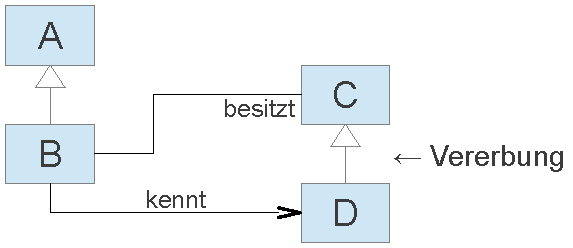
\includegraphics[width=0.7\linewidth]{images/uml-intro.pdf}
		\end{center}
	\end{block}
\end{frame}

\begin{frame}{Wichtige Entwurfsmuster I}
	\begin{block}{Adapter}
		Übersetzt inkompatible Schnittstellen
		\vspace{-0.7em}
		\begin{center}
			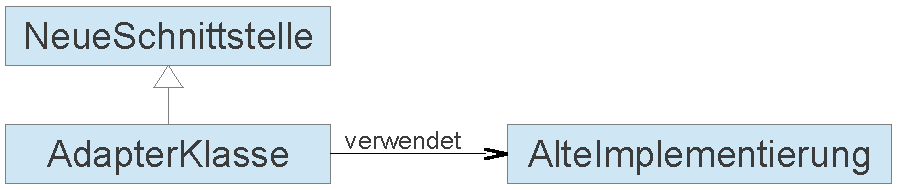
\includegraphics[width=0.85\linewidth]{images/adapter.pdf}
		\end{center}
	\end{block}
	
	\begin{block}{Proxy/Decorator/Wrapper}
		Wird einer anderen Instanz vorgeschaltet und kann diese so kontrollieren oder ihre Funktionalität erweitern		
		\vspace{-0.7em}
		\begin{center}
			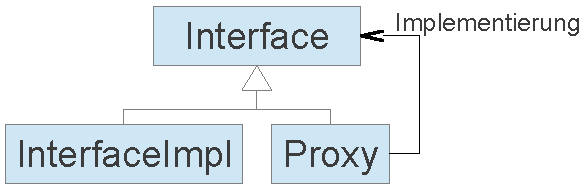
\includegraphics[width=0.6\linewidth]{images/proxy.pdf}
		\end{center}
	\end{block}
\end{frame}
	
\begin{frame}{Wichtige Entwurfsmuster II}
	\begin{block}{Bridge/Pointer to Implementation (Pimpl)}
		Ermöglicht das Entkoppeln von Schnittstelle und Implementierung und erlaubt es, letztere zu verbergen (Information hiding!)
		\vspace{-0.7em}
		\begin{center}
			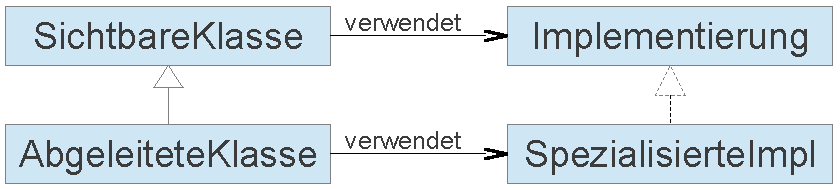
\includegraphics[width=0.85\linewidth]{images/bridge.pdf}
		\end{center}
		\vspace{-1em}
		Implementierungsdetails (\texttt{private}-Bereich!) werden unsichtbar, es bleibt nur ein Zeiger auf eine anonyme Klasse.
		\vspace{-0.5em}		
		\lstinputlisting[basicstyle=\tiny]{cpp-code/pimpl.cpp}
	\end{block}
\end{frame}
	
\begin{frame}{Wichtige Entwurfsmuster III}
	\begin{block}{Observer}
		\begin{itemize}
			\item Benachrichtigung anderer Komponenten über Ereignisse
			\item Die konkreten Implementierungen müssen/sollen sich dabei nicht kennen
		\end{itemize}
		\vspace{-0.7em}
		\begin{center}
			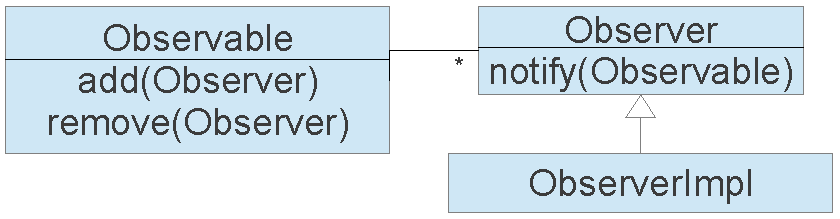
\includegraphics[width=0.85\linewidth]{images/observer.pdf}
		\end{center}
		Sonderfall: Vermittler (Mediator) ähnelt dem Observer
	\end{block}
\end{frame}
	
\begin{frame}{Wichtige Entwurfsmuster IV}
	\begin{block}{Template (Schablonenmethode) und Strategie}
		\begin{itemize}
			\item Schablonenmethoden delegieren die Implementierung einzelner Aspekte an Kindklassen
			\item Das Strategie-Pattern macht komplette Klassen als Gegenstand einer Implementierung austauschbar
		\end{itemize}
		\vspace{-1em}
		\begin{center}
			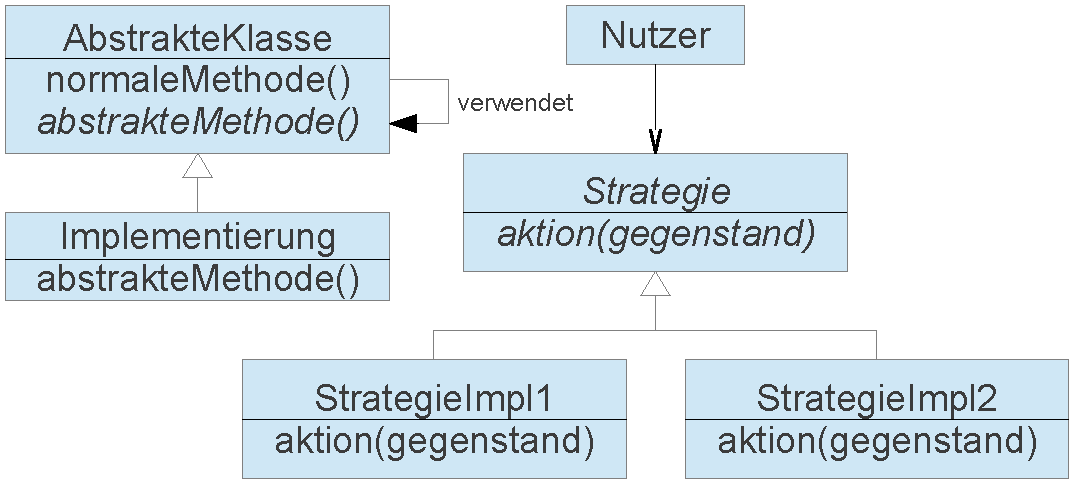
\includegraphics[width=0.85\linewidth]{images/strategy.pdf}
		\end{center}
	\end{block}
\end{frame}

\begin{frame}{Wichtige Entwurfsmuster V}	
	\begin{block}{Factory}
		\begin{itemize}
			\item Klassen oder Methoden, die neue Objekte erzeugen
			\item Interpretierbar als Sonderfall von Template und Strategie
		\end{itemize}		
		\vspace{-1em}
		\begin{center}
			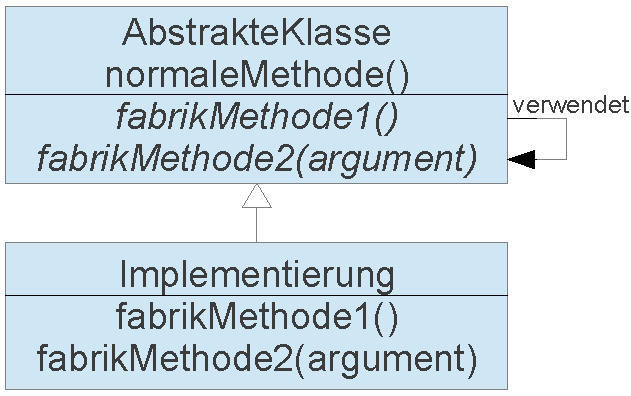
\includegraphics[width=0.6\linewidth]{images/factorymethod.pdf}
		\end{center}		
	\end{block}
\end{frame}

\begin{frame}{Wichtige Entwurfsmuster V}	
	\begin{block}{Abstrakte Factory}
		\begin{center}
			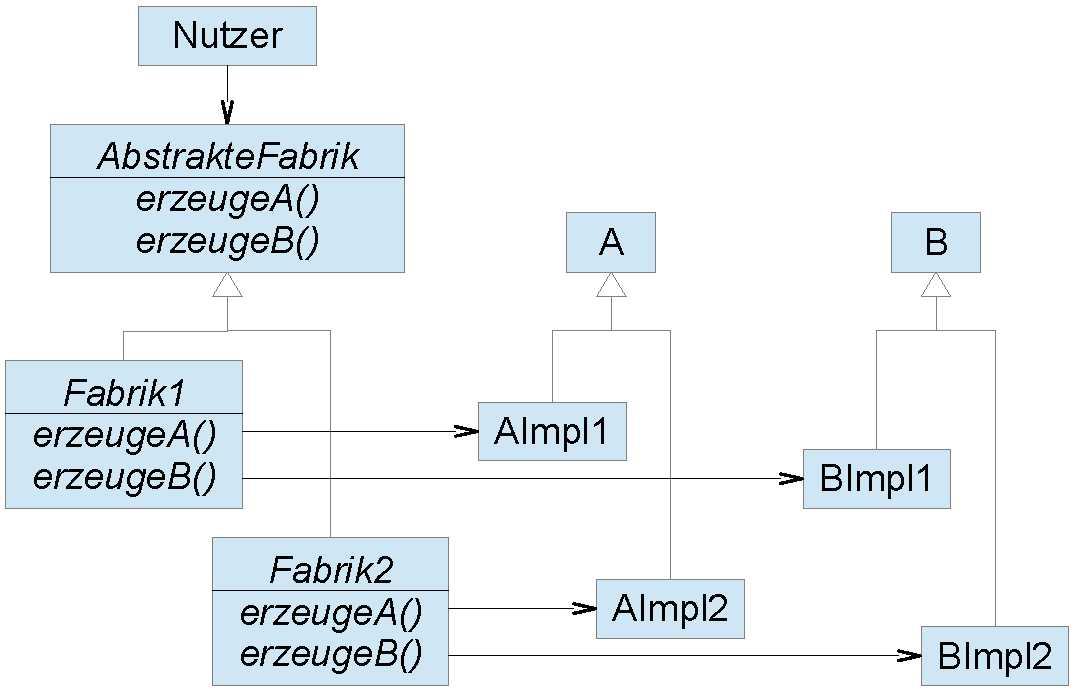
\includegraphics[width=0.85\linewidth]{images/factory.pdf}
		\end{center}		
	\end{block}
\end{frame}

\begin{frame}{Wichtige Entwurfsmuster VI}
	\begin{block}{Fassade}
		Eine Klasse die das (komplizierte) Zusammenspiel innerhalb eines ganzen Subsystems hinter einer einfachen, einheitlichen Schnittstelle verbirgt.
	\end{block}
	
	\begin{block}{Dummy/Null-Objekt}
		Eine Klasse die einfach \enquote{nichts} tut. Solche Objekte können aufwändige Sonderfälle ersetzen.
	\end{block}
\end{frame}



\section{Praxis}
\begin{frame}[fragile]{Praxis!}
	\begin{itemize}
		\item Bearbeitung der Aufgaben aus den letzten Workshops
	\end{itemize}
	\ \\
	\ \\
	\large{\url{https://github.com/kit-cpp-workshop/workshop-ss12-11}} \\
	\ \\
	Aufgabenbeschreibungen und Hinweise: Siehe \verb|README.md|

\end{frame}


\end{document}
